\chapter{Results}

\todo{Deep architectures in PCP: \cite{di2012deep}}

\section{Hyper-Parameter Optimization}

\section{Model evaluation on the different benchmark sets}

    \begin{table}[H]
        \centering
        \resizebox{\textwidth}{!}{
        \begin{tabular}{|l|ccc|ccc|ccc|}
            \hline
            & & CASP11 & & & CAMEO & & & Membrane & \\
            \hline
            Method & Short & Medium & Long & Short & Medium & Long & Short & Medium & Short \\
            \hline
            \hline
            Wynona & - & - & - & - & - & - & - & - & - \\
            PconsC3 & 0.25 & 0.29 & 0.40 & 0.21 & 0.23 & 0.27 & 0.15 & 0.9 & 0.33 \\  % 0.9?
            RaptorX-Contact & 0.28 & 0.35 & 0.55 & 0.23 & 0.28 & 0.42 & 0.16 & 0.22 & 0.47 \\
            MetaPSICOV & 0.26 & 0.31 & 0.39 & 0.22 & 0.22 & 0.28 & 0.16 & 0.21 & 0.35 \\
            PlmDCA & 0.14 & 0.16 & 0.27 & 0.11 & 0.13 & 0.19 & 0.08 & 0.11 & 0.21 \\
            PSICOV & 0.14 & 0.15 & 0.24 & 0.13 & 0.14 & 0.18 & 0.09 & 0.11 & 0.20 \\
            mfDCA & 0.13 & 0.15 & 0.22 & 0.10 & 0.11 & 0.15 & 0.09 & 0.12 & 0.24 \\
            \hline
        \end{tabular}
        }
        \captionof{table}{Best-L/5 PPV of different methods on short,
        medium and long-range contacts. Results are shown for the three
        different benchmark sets: CASP11 targets, CAMEO proteins, and
        the benchmark set of membrane proteins.}
        \label{benchmark}
    \end{table}

    \subsection{CASP11}

        \todo{}

    \subsection{CAMEO}

        \todo{}

    \subsection{Membrane proteins}

        \todo{}

\section{Sensitivity to the number of homologous sequences}

    \begin{figure}[H]
        \begin{center}
            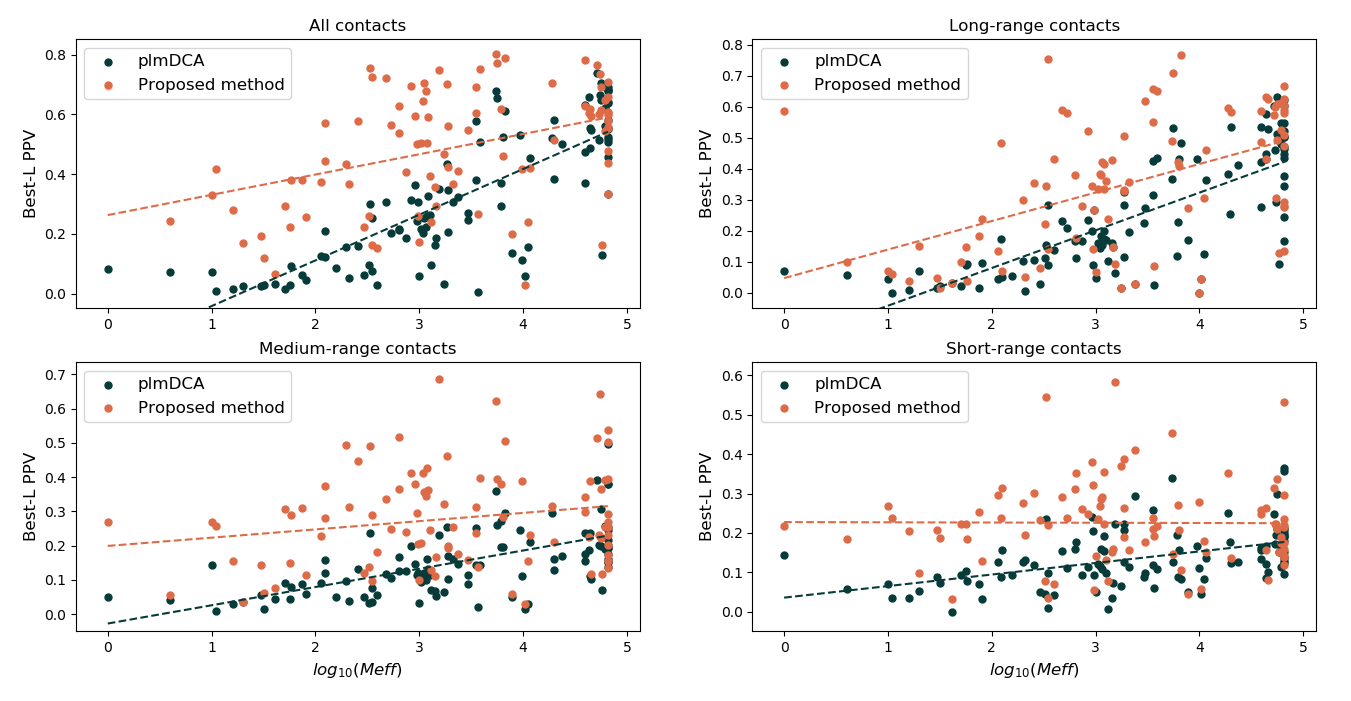
\includegraphics[width=\textwidth, keepaspectratio]{imgs/Meff.png}
            \caption{Performance as a function of the logarithm of the effective
            number of homologous sequences. Top figure shows the results on
            CASP11 targets for all contacts. Bottom left and bottom right figures
            focus on medium-range and long-range contacts, respectively.}
            \label{sensitivity}
        \end{center}
    \end{figure}

\section{Folding proteins from contact maps}

    \begin{figure}[H]
        \begin{center}
            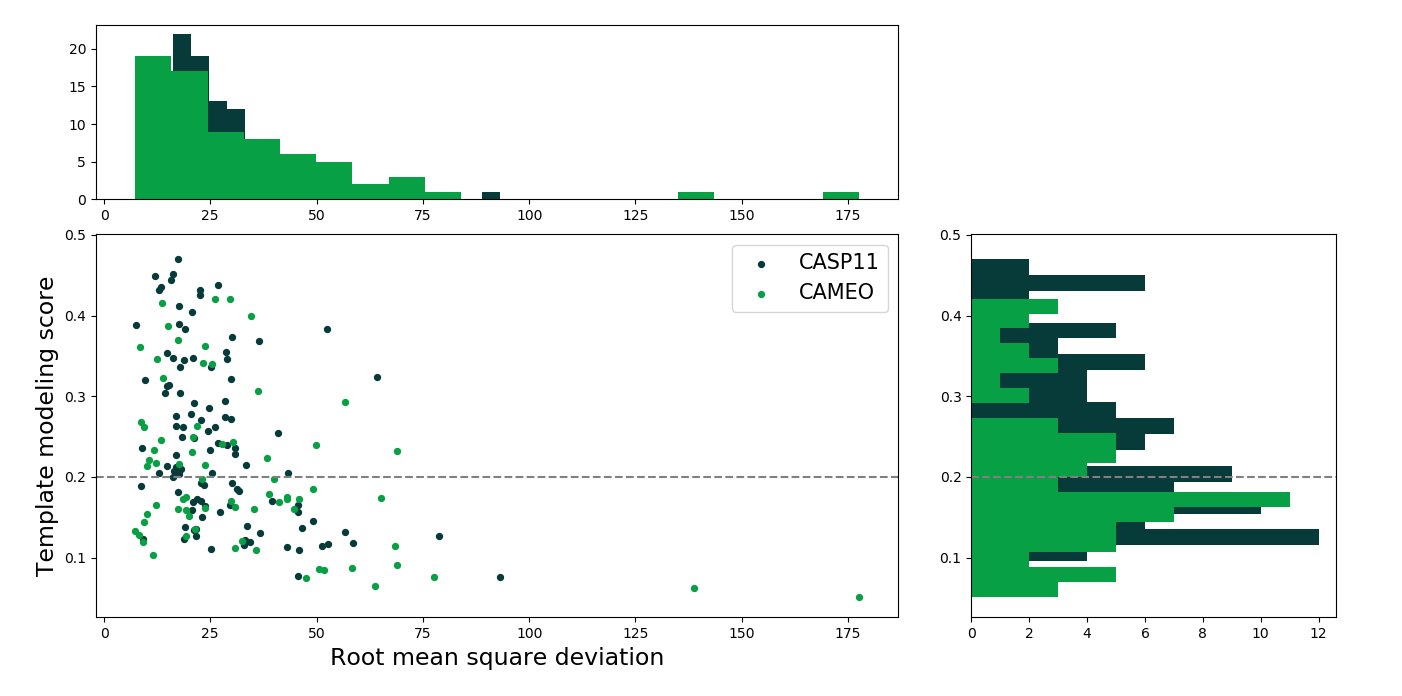
\includegraphics[width=\textwidth, keepaspectratio]{imgs/fold.png}
            \caption{Root mean square deviations and template-modelling scores
            on the 3 benchmark sets.}
            \label{fold}
        \end{center}
    \end{figure}

\todo{tSNE: \cite{Maaten2008VisualizingDU}}
